% =========================================================================
% Capítulo 1 - Tema 02: Cinemática en Coordenadas Esféricas
% =========================================================================

\section{Tema 02: Cinemática en Coordenadas Esféricas}

Las coordenadas esféricas son naturales para problemas con simetría central,
como el movimiento de péndulos esféricos o trayectorias sobre superficies curvas.

\subsection{Ejercicios}

\subsubsection{Problema: Anillo rotador}
Un anillo \( P \) se desliza a lo largo de un aro circular de radio \( r \) como indica la figura \ref{fig:anillo_deslizante}. El aro rota con una velocidad angular \( \Omega \) que apunta en la dirección vertical gracias a las uniones en \( A \) y \( B \), que en conjunto actúan como una conexión de revolución.

Si el ángulo \( \phi \) describe la posición del anillo con respecto al centro \( O \) del aro circular, determine:

\begin{enumerate}
    
    \item Marcos de referencia y Sistemas de coordenadas.
    \item La posición del anillo \( P \).
    \item La velocidad y aceleración angular del anillo \( P \).
    \item La velocidad y aceleración del anillo \( P \) vistos por un observador fijo en \( O \).
\end{enumerate}

\begin{figure}[!ht]
    \centering
    \begin{tikzpicture}[>=Latex, scale=1]
        % --- Parámetros Geométricos ---
        \pgfmathsetmacro{\Rout}{2.2} % Radio exterior del anillo
        \pgfmathsetmacro{\Rin}{2.0}  % Radio interior del anillo
        \pgfmathsetmacro{\Rmid}{(\Rin+\Rout)/2} % Radio medio (para P)
        \def\ThetaAngle{50}             % Ángulo theta desde la vertical

        \coordinate (O) at (0,0);

        % --- 1. Eje Central y Centro ---
        \draw[dash dot, thin] (0, -\Rout - 1.5) -- (0, \Rout + 1.8);
        \filldraw (O) circle (1.5pt) node[left, xshift=-2pt] {$O$};

        % --- 2. Anillo Circular ---
        % Relleno gris entre dos círculos para dar grosor (even odd rule)
        \draw[fill=gray!35, thick, even odd rule] (O) circle (\Rout) (O) circle (\Rin);

        % --- 3. Soporte Superior A ---
        \begin{scope}[shift={(0, \Rout)}]
            % Pieza en T (móvil, unida al anillo)
            \draw[fill=gray!50, thick] (-0.15, 0) rectangle (0.15, 0.3);
            \draw[fill=gray!50, thick] (-0.4, 0.3) rectangle (0.4, 0.6);
            % Guía Fija (C negra)
            \draw[fill=black] (-0.6, 0.2) rectangle (0.6, 0.7);
            \draw[fill=white, thick] (-0.42, 0.18) rectangle (0.42, 0.62);
            % Techo fijo (rayado)
            \draw[thick, pattern=north east lines] (-0.7, 0.7) rectangle (0.7, 1.0);
            \draw[thick] (-0.7, 0.7) -- (0.7, 0.7);
            \node[left] at (-0.6, 0.35) {$A$};
        \end{scope}

        % --- 4. Soporte Inferior B (Espejo de A) ---
        \begin{scope}[shift={(0, -\Rout)}, rotate=180]
            \draw[fill=gray!50, thick] (-0.15, 0) rectangle (0.15, 0.3);
            \draw[fill=gray!50, thick] (-0.4, 0.3) rectangle (0.4, 0.6);
            \draw[fill=black] (-0.6, 0.2) rectangle (0.6, 0.7);
            \draw[fill=white, thick] (-0.42, 0.18) rectangle (0.42, 0.62);
            \draw[thick, pattern=north east lines] (-0.7, 0.7) rectangle (0.7, 1.0);
            \draw[thick] (-0.7, 0.7) -- (0.7, 0.7);
            \node[left] at (0.6, 0.35) {$B$};
        \end{scope}

        % --- 5. Partícula P ---
        % Posición calculada para estar en el medio del grosor del anillo
        \coordinate (P) at ({90-\ThetaAngle}:\Rmid);
        \begin{scope}[shift={(P)}, rotate={90-\ThetaAngle}]
            \draw[fill=gray!40, thick, rounded corners=2pt] (-0.2, -0.12) rectangle (0.2, 0.12);
            \node[above right, xshift=2pt] {$P$};
        \end{scope}

        % --- 6. Vectores y Ángulos ---
        % Vector Posición r
        \draw[->, thick] (O) -- (P) node[midway, right] {$r$};
        % Ángulo Theta desde la vertical
        \draw[->, thick] (0, 1.0) arc (90:{90-\ThetaAngle}:1.0);
        \node at ({90-\ThetaAngle/2}:1.3) {$\theta$};

        % Vector Rotación Omega (Superior)
        \coordinate (TopAxis) at (0, \Rout + 1.3);
        \draw[->, very thick] (TopAxis) -- ++(0, 0.8); 
        \draw[->, thick] ($(TopAxis)+(-0.3,0.3)$) arc (170:370:0.4 and 0.15);
        \node[left] at ($(TopAxis)+(-0.5, 0.4)$) {$\Omega$};

    \end{tikzpicture}
    \caption{Sistema mecánico compuesto por un anillo circular giratorio con soportes deslizantes en $A$ y $B$. La partícula $P$ se desplaza a lo largo del anillo con una posición definida por $r$ y $\theta$.}
    \label{fig:anillo_deslizante}
\end{figure}

\ifmostrarSolucion
\begin{tcolorbox}[title=Anillo rotador,breakable]
\textbf{Marcos de referencia y Sistemas de coordenadas}\\

Lo primero de todo es podes obtener los marcos de referencia y se parte primero con el marco de referencia inercia;\\
En este caso se puede apreciar como parece un sistemas de coordenadas esférico, pero para analizar este sistemas de coordenadas lo que haremos sera un sistema doble cilíndrico, el primero asociado al aro, el el segundo en el aro asociado al anillo, en realidad es así como se define un sistema de coordenadas esférico, a base de dos cilíndricos, uno sobre el otro.
\begin{itemize}
    \item $\mathcal{N}$ El suelo $\longrightarrow\{\vec{E}_x;\vec{E}_y;\vec{E}_z\}$
    \item $\mathcal{A}$ El aro $\longrightarrow\{\vec{e}_x;\vec{e}_y;\vec{e}_z\}$
    \item $\mathcal{B}$ El anillo $\longrightarrow\{\vec{e}_r;\vec{e}_\theta;\vec{e}_\phi\}$
\end{itemize}

En este caso se pueden apreciar 2 sistemas de coordenadas el del marco inercial, y el del marco de referencia $\mathcal{A}$, donde los puntos grises son el anillo cortado. Aparte notar que en la figura \ref{fig:D1} $\Omega$ no es el angulo por si mismo si no que es la velocidad angular de un marco respecto otro


\begin{center}
    % --- INICIO FIGURA 2 ---
    \begin{minipage}{0.48\textwidth}
        \centering
        \begin{tikzpicture}[>=Stealth, scale=1.3]
            % Definición de radio y ángulos
            \def\R{1.6}
            \def\angOmega{55}
            
            % Ejes principales negros
            \draw[<->, thick] (-1.8,0) -- (2.0,0);
            \draw[<->, thick] (0,-1.8) -- (0,2.0);
            
            % Círculo
            \draw (0,0) circle (\R);
            
            % Masas (Puntos grises en el anillo)
            \fill[gray] (\angOmega:\R) circle (3pt);
            \fill[gray] (\angOmega+180:\R) circle (3pt);
            
            % Sistema fijo (Azul)
            \draw[->, blue!70!black, thick] (0,0) -- (1.2,0) node[below right] {$\vec{E}_x$};
            \draw[->, blue!70!black, thick] (0,0) -- (0,1.2) node[above left] {$\vec{E}_y$};
            
            % Sistema móvil (Verde)
            \draw[->, green!40!black, thick] (0,0) -- (\angOmega:1.2) node[above left= -2pt] {$\vec{e}_x$};
            \draw[->, green!40!black, thick] (0,0) -- ({\angOmega+90}:1.2) node[left=2pt] {$\vec{e}_y$};
            
            % Punto P
            \fill (\angOmega:1.2) circle (1.5pt) node[right=2pt] {P};
            
            % Ángulo Omega
            \draw[->] (0.7,0) arc (0:\angOmega:0.7) node[midway, right=1pt] {$\Omega$};
            
            % Origen (Punto saliendo)
            \fill[white] (0,0) circle (4pt);
            \draw (0,0) circle (4pt);
            \fill (0,0) circle (1.5pt);
            \node[below left=2pt] at (0,0) {$\vec{E}_z = \vec{e}_z$};
            
            % Falso Caption
            \vspace{0.5cm}
            \node[below, align=center, text width=6cm] at (0,-2) 
                {\footnotesize \textbf{Figura 2:} Diagrama de corte del anillo};
        \end{tikzpicture}
    \end{minipage}\hfill
    % --- INICIO FIGURA 3 ---
    \begin{minipage}{0.48\textwidth}
        \centering
        \begin{tikzpicture}[>=Stealth, scale=1.3]
            % Definición de radio y ángulos
            \def\R{1.6}
            \def\angTheta{30} % Ángulo desde la horizontal (equivale a theta desde el eje z)
            
            % Ejes principales negros
            \draw[<->, thick] (-1.8,0) -- (2.0,0);
            \draw[<->, thick] (0,-1.8) -- (0,2.0);
            
            % Círculo
            \draw (0,0) circle (\R);
            
            % Sistema marco A (Verde)
            \draw[->, green!40!black, thick] (0,0) -- (1.2,0) node[below right] {$\vec{e}_x$};
            \draw[->, green!40!black, thick] (0,0) -- (0,1.2) node[above left] {$\vec{e}_z$};
            
            % Sistema marco B (Café/Rojo)
            \draw[->, red!40!black, thick] (0,0) -- (\angTheta:1.2) node[above left= -2pt] {$\vec{e}_r$};
            \draw[->, red!40!black, thick] (0,0) -- ({\angTheta-90}:1.2) node[below left] {$\vec{e}_\theta$};
            
            % Punto P en el anillo
            \fill (\angTheta:\R) circle (1.5pt) node[right=2pt] {P};
            
            % Ángulo Theta (Desde e_z hasta e_r)
            \draw[<->] (0,0.8) arc (90:\angTheta:0.8) node[midway, above right=1pt] {$\theta$};
            
            % Origen (Cruz entrando)
            \fill[white] (0,0) circle (4pt);
            \draw (0,0) circle (4pt);
            \draw (-2.5pt,-2.5pt) -- (2.5pt,2.5pt);
            \draw (-2.5pt,2.5pt) -- (2.5pt,-2.5pt);
            \node[below left=2pt] at (0,0) {$\vec{e}_y = \vec{e}_\phi$};
            
            % Falso Caption
            \vspace{0.5cm}
            \node[below, align=center, text width=6cm] at (0,-2) 
                {\footnotesize \textbf{Figura 1} Sist. Coord. marcos $\mathcal{A}, \mathcal{B}$};
        \end{tikzpicture}
    \end{minipage}
\end{center}

\textbf{La posición del anillo \( P \).}\\
Para obtener la posición siempre la tomamos desde un punto inercial (basicamente un punto que no se mueva) por ejemplo el centro  $O$, como también lo podría ser el punto $A$ en este caso demostraremos que da lo mismo el punto que elijamos mientras sea inercial.
$$\vec{r}_{P/A}=\underbrace{\vec{r}_{P/O}}_{r\vec{e}_r} +\underbrace{\vec{r}_{O/A}}_{-r\vec{e}_z}$$

\textbf{La velocidad y aceleración angular del anillo \( P \).}\\
Para este caso se tiene que analizar la velocidad angular se tiene que ver respecto a que ejes son los que giran los marcos de referencia, rapidamente podemos darnos cuenta que $\mathcal{A}$ gira con velocidad $\Omega$ gira con respecto al $\vec{e}_z$ o $\vec{E}_z$ que son el mismo vector, y junto a \ref{fig:D2} se puede ver que el marco de referencia $\mathcal{B}$ gira respecto al $\mathcal{A}$ con velocidad angular $\dot\theta$ en $\vec{e}_{\phi}$, siempre recordar de usar la regla de la mano derecha para saber si es que es positivo o negativo el vector.
$$\velang{N}{A}=\Omega\vec{e}_z$$
$$\velang{A}{B}=\dot\theta\vec{e}_y$$
Pero lo que queremos obtener es la velocidad angular del marco referencia del anillo y lo que tenemos es la del anillo respecto al aro ($\velang{A}B$) y la del aro respecto al suelo $\velang{N}{A}$, pero la velocidad angular cumple la propiedad aditiva, (no se cumple para la aceleración angular.)
$$\velang{N}{B}=\velang{N}{A}+\velang{A}{B}=\dot\theta\vec{e}_y+\Omega\vec{e}_z$$
Ahora solo falta la aceleración angular que se define como 
$$\accang{N}{F} =\der{}{N}\left(\velang{N}{F}\right)$$ ($\mathcal{F}$ es un ejemplo simplemente)\\

Entonces podemos calcularlo

$$\accang{N}{B} =\der{}{N}\left(\velang{N}{B}\right)$$
En este caso decidimos calcularlo respecto al marco $\mathcal{A}$ porque ambos vectores están en fijos a ese marco

$$\accang{N}{B}=\transporta{\velang{N}{B}}{N}{A}$$
$$\accang{N}{B}=\transporta{\left(\dot\theta\vec{e}_y+\Omega\vec{e}_z\right)}{N}{A}$$
$$\accang{N}{B}=\dot\theta\vec{e}_y+\dot\Omega\vec{e}_z-\Omega\dot\theta\vec{e}_x$$
\textbf{La velocidad y aceleración del anillo \( P \) vistos por un observador fijo en \( O \).}
Si bien en este caso dice que sea desde el punto $O$ (deberiamos hacerlo desde $O$) el; hacerlo de cualquier punto (Observador) fijo  también sirve.

$$\marc{\vec{v}_P}{N}=\der{\vec{r}_{P/A}}{N}=\der{(r\vec{e}_r-r\vec{e}_z)}{N}$$
Por propiedades de la derivada podemos separar por la suma y obtenemos
$$\der{\vec{r}_{P/A}}{N}=\der{\vec{r}_{P/O}}{N}+\der{\vec{r}_{O/A}}{N}$$
$$\der{\vec{r}_{O/A}}{N}=\der{(-r\vec{e}_z)}{N}=\transporta{(-r\vec{e}_z)}{N}{A}$$
$$\der{(-r\vec{e}_z)}{A}=\vec{0} \quad\quad \velang{N}{A}\times(-r\vec{e}_z)=\vec{0}$$
Ahora falta $\vec{r}_{P/O}$ (que en este caso usaremos el teorema del transporte respecto a $\mathcal{B}$ ya que tenemos el vector posición en base de $\mathcal{B}$)
$$\der{\vec{r}_{P/O}}{N}=\transporta{(r\vec{e}_r)}{N}{B}$$
$$\der{(r\vec{e}_r)}{B}=\vec{0} \quad\quad \velang{N}{B}\times(r\vec{e}_r)=\left(\dot\theta\vec{e}_y+\Omega\vec{e}_z\right)\times(r\vec{e}_r)$$
Aquí tenemos un problema, no todos los vectores están en la misma base, no sabemos cuanto es $\vec{e}_z\times \vec{e}_r$ paras esto transformaremos el vector $\vec{e}_z$ en la base asociada al marco $\mathcal{B}$

$$\vec{e}_z=\cos{(\theta)}\vec{e}_r-\sin(\theta)\vec{e}_\theta$$
$$\vec{e}_x=\sin{(\theta)}\vec{e}_r+\cos(\theta)\vec{e}_\theta$$
$$\vec{e}_y=\vec{e}_\phi$$
Recuerden siempre que trabajamos tenemos que descomponer el vector completo, no sirve que solo nos quedemos con una componente, para confirmar que es el vector completo se puede sacar la norma y debería dar siempre 1.\\

Ahora que ya tenemos la transformación de $\vec{e}_z$ podemos terminar de calcular la velocidad
$$\der{(r\vec{e}_r)}{B}=\vec{0} $$
$$\velang{N}{B}\times(r\vec{e}_r)=\left(\dot\theta\vec{e}_\phi+\Omega(\cos{(\theta)}\vec{e}_r-\sin(\theta)\vec{e}_\theta))\right)\times(r\vec{e}_r)=r\dot\theta\vec{e}_\theta +r\Omega\sin{(\theta)}\vec{e}_\phi$$

\textbf{Aceleración}\\
Ahora simplemente toca hacer los mismos pasos para la aceleración
$$\der{\marc{}{N}\vec{v}_P}{N}=\transporta{\left(r\dot\theta\vec{e}_\theta +r\Omega\sin{(\theta)}\vec{e}_\phi\right)}{N}{B}$$
$$\der{\left(r\dot\theta\vec{e}_\theta +r\Omega\sin{(\theta)}\vec{e}_\phi\right)}{B}=r\ddot{\theta}\vec{e}_\theta+r\dot\Omega\sin{(\theta)}\vec{e}_\phi+r\Omega\dot\theta\cos{(\theta)}\vec{e}_{\phi}$$

$$\velang{N}{B}\times\left(\marc{\vec{v}}{N}\right)=\left(\dot\theta\vec{e}_\phi+\Omega(\cos{(\theta)}\vec{e}_r-\sin(\theta)\vec{e}_\theta))\right)\times\left(r\dot\theta\vec{e}_\theta +r\Omega\sin{(\theta)}\vec{e}_\phi\right)=$$
$$=r\dot\theta^2 \vec{e}_r+\vec{0}+r\dot\theta\Omega\cos(\theta)\vec{e}_\phi+r\Omega^2\cos(\theta)\sin(\theta)(-\vec{e}_\theta)+r\dot\theta\Omega(-\sin(\theta))\vec{e}_{\phi}-r\Omega^2\sin^2(\theta)(\vec{e}_r)$$

$$\marc{\vec{a}}{N}=\left(-r\dot\theta^2-r\Omega^2\sin^2(\theta)\right)\vec{e}_r+\left(r\ddot{\theta}-r\Omega\sin(\theta)\cos(\theta)\right)\vec{e}_\theta+\left(r\dot\Omega\sin(\theta)+2r\Omega\dot\theta\cos(\theta)\right)\vec{e}_\phi$$

\end{tcolorbox}
\fi

\subsubsection{Curva espiral en coordenadas esféricas}

Considere una curva espiral descrita en coordenadas esféricas por las ecuaciones:
\[ r = R, \quad \theta = N\phi \]
donde $R$ y $N$ son constantes conocidas ($N$ entero par). Una partícula se mueve sobre la espiral partiendo desde el extremo superior ($\phi=0$) y manteniendo una velocidad angular cenital constante y conocida, $\dot{\phi} = \omega_0$. Se pide:

\begin{enumerate}
    \item Utilizando coordenadas esféricas, escriba los vectores velocidad y aceleración para una posición arbitraria de la partícula sobre su trayectoria.
    \item Determine el valor del radio de curvatura de la trayectoria en el ecuador ($\phi = \frac{\pi}{2}$).
    \item Encuentre una expresión para la longitud total de la espiral y para el tiempo que la partícula tarda en recorrerla.
\end{enumerate}

\begin{figure}[!ht]
    \centering
    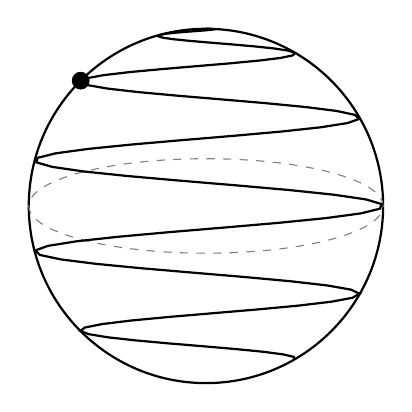
\begin{tikzpicture}[scale=1.5]
        % --- 1. Esfera (Contorno) ---
        \draw[thick] (0,0) circle (1.5);
        \draw[dashed, gray] (0,0) ellipse (1.5 and 0.4); % Ecuador

        % --- 2. Dibujo de la Espiral (Simulada) ---
        \draw[thick, samples=100, domain=0:10*pi] 
            plot ({1.5*sin(deg(\x/12))*cos(deg(\x))}, {1.5*cos(deg(\x/12))});
            
        % --- 3. Partícula ---
        \filldraw ({1.5*sin(deg(pi/4))*cos(deg(3*pi))}, {1.5*cos(deg(pi/4))}) circle (2pt);
    \end{tikzpicture}
    \caption{Trayectoria espiral sobre una superficie esférica de radio $R$.}
\end{figure}
\subsubsection{Péndulo esférico}

Una partícula $P$ está suspendida de un extremo de una varilla rígida de longitud $L$. La posición se describe con ángulos esféricos $\theta$ y $\phi$ respecto a una base fija $\{E_x, E_y, E_z\}$, donde $E_z$ apunta hacia abajo.

Se pide determinar para un observador fijo al suelo:
\begin{enumerate}
    \item Los marcos de referencia y sistemas de coordenadas.
    \item El vector posición de la partícula $P$.
    \item El vector velocidad angular de la varilla.
    \item Los vectores de velocidad y aceleración de la partícula.
\end{enumerate}

\begin{figure}[!ht]
    \centering
    \begin{tikzpicture}[
        >=Latex, 
        x={(1cm,0cm)}, 
        y={(-0.4cm,-0.3cm)}, % Perspectiva ajustada para claridad
        z={(0cm,-1cm)},      % Eje Z apuntando hacia abajo
        scale=2.5
    ]
        % --- Parámetros ---
        \def\L{2.0}       % Longitud varilla
        \def\thetaAng{35} % Ángulo theta ( plano horizontal)
        \def\phiAng{40}   % Ángulo phi (respecto a la vertical)
        \def\arcRad{0.7}  % Radio para los arcos de ángulo

        % --- Coordenadas ---
        \coordinate (O) at (0,0,0);
        
        % Cálculo de P en coordenadas esféricas (Z hacia abajo)
        \pgfmathsetmacro{\Px}{\L*sin(\phiAng)*cos(\thetaAng)}
        \pgfmathsetmacro{\Py}{\L*sin(\phiAng)*sin(\thetaAng)}
        \pgfmathsetmacro{\Pz}{\L*cos(\phiAng)}
        \coordinate (P) at (\Px, \Py, \Pz);
        \coordinate (Q) at (\Px, \Py, 0); % Proyección en plano XY

        % --- 1. Soporte y Ejes ---
       \begin{scope}[canvas is xy plane at z=0]
            \fill[pattern=north east lines] (0,0) circle (0.15);
            \draw[thick] (0,0) circle (0.15);
        \end{scope}
        \filldraw (O) circle (0.8pt) node[above left] {$O$};

        % Ejes
        \draw[->, thick] (O) -- (1.8,0,0) node[right] {$E_x$};
        \draw[->, thick] (O) -- (0,1.8,0) node[left] {$E_y$};
        \draw[->, thick, -{Latex[length=3mm]}] (O) -- (0,0,2.2) node[below] {$E_z$};

        % --- 2. Proyecciones y Varilla ---
        \draw[dashed, thin, gray!70] (O) -- (Q);
        \draw[dashed, thin, gray!70] (Q) -- (P);
        \draw[dashed, thin, gray!70] (P) -- (0,0,\Pz); % Proyección al eje Z

        % Varilla y Partícula
        \draw[line width=1.5pt, color=gray!70] (O) -- (P) node[midway, right, xshift=2pt] {$L$};
        \filldraw[shading=ball, ball color=gray!40] (P) circle (3pt) node[right, xshift=4pt] {$P$};
        \filldraw[gray] (Q) circle (1pt) node[right] {$Q$};

        % --- 3. Ángulos (CORREGIDOS EN 3D) ---
        
        % Ángulo Theta (Plano XY, es más fácil)
        \draw[->, thin] (\arcRad,0,0) arc (0:\thetaAng:\arcRad);
        \node at ({(\arcRad+0.2)*cos(\thetaAng/2)}, {(\arcRad+0.2)*sin(\thetaAng/2)}, 0) {$\theta$};

        % --- CORRECCIÓN DEL ÁNGULO PHI ---
        % Calculamos 3 puntos en el espacio para dibujar el arco 3D correcto
        % 1. Inicio sobre el eje Ez
        \coordinate (PhiStart) at (0, 0, \arcRad);
        % 2. Fin sobre la varilla OP (P escalado)
        \coordinate (PhiEnd) at ($ (O)!{\arcRad/\L}!(P) $);
        % 3. Un punto intermedio para la curvatura (aprox. a la mitad del ángulo)
        \pgfmathsetmacro{\halfPhi}{\phiAng/2}
        \coordinate (PhiMid) at (
            {\arcRad*sin(\halfPhi)*cos(\thetaAng)},
            {\arcRad*sin(\halfPhi)*sin(\thetaAng)},
            {\arcRad*cos(\halfPhi)}
        );

        % Dibujamos la curva suave pasando por los 3 puntos 3D
        \draw[->, thin] plot [smooth] coordinates {(PhiStart) (PhiMid) (PhiEnd)};
        
        % Etiqueta Phi posicionada cerca del punto medio
        \node at ($(PhiMid) + (0,0,0.2)$) {$\phi$};

    \end{tikzpicture}
    \caption{Esquema del péndulo esférico con la representación correcta del ángulo $\phi$ en el espacio 3D.}
    \label{fig:pendulo_esferico_corregido}
\end{figure}
